\subsection{End-to-end case study: building a text-based equity factor}

% 
% Version: 3.2.1
% Last updated: 2026-07-20
% Provenance: fifth and final chapter of Part V of the 2nd edition, extracted from
% the monolithic Chapter_20_Draft19.md (v3.9.7, archived in
% `_archive_monolithic_v3.9.7/`).
%

\subsubsection{Introduction}

Chapters 20 through 23 developed the four generations of NLP methods and the factor families each generation produces, but the empirical evaluations in those chapters were necessarily piecemeal: each method was demonstrated against the most natural baseline for its own paradigm, on the case-study universe but without the full portfolio-construction machinery that the book develops for traditional factor portfolios. This closing chapter of Part V brings the full pipeline together. We work through the practical considerations that every production text-factor pipeline must address, define the case study, construct features that span the methods of the preceding chapters, train and validate a model, run a backtest following the Chapter 12 protocol, and report the result in full, including the conditions under which the headline finding does and does not survive transaction costs.

The classical, embedding, transformer, and LLM methods of Chapters 20 through 23 are tools; the case study below shows what those tools produce when applied with discipline to the book's standard universe.

\subsubsection{Model selection and validation}

The choice of NLP model depends on the application, the available labeled data, and the computational budget. A useful hierarchy is:

\begin{enumerate}
\item \textbf{Dictionary methods} (Loughran-McDonald): fast, transparent, no training required. Suitable when the text is formulaic and the signal is well-understood.
\item \textbf{Fine-tuned BERT/FinBERT} (Chapter 22): moderate compute, requires labeled data. Best for classification tasks (sentiment, topic) where labeled examples are available.
\item \textbf{LLM with prompting} (Chapter 23): high compute, no training required. Best for complex tasks (summarization, reasoning, multi-label classification) or when labeled data is scarce.
\item \textbf{Fine-tuned LLM}: highest compute. Best when task-specific performance must be maximized and sufficient labeled data and compute are available.
\end{enumerate}

Validating NLP outputs for financial relevance requires more than standard ML metrics (accuracy, F1). A sentiment model might achieve 90\% accuracy on a benchmark dataset but produce signals with zero predictive power for returns. The ultimate validation is the out-of-sample portfolio performance of the resulting factor, not the NLP model's classification accuracy. For a broader methodological tour of this model hierarchy, from bag-of-words through learned classifiers and the validation traps specific to financial language, we refer the reader to the \textit{Journal of Accounting Research} survey of \cite{loughran2016textual}, which remains the most widely cited methodological reference in the area.

\subsubsection{Backtesting and timestamp discipline}

Backtesting NLP-based strategies introduces unique challenges beyond those discussed in Chapter 12.

\textbf{Timestamp discipline.} The most critical issue is \textit{look-ahead bias}. Financial text has a publication timestamp, and the NLP signal must be constructed using only information available at the time of portfolio formation. For example, a 10-K filing typically becomes available on EDGAR several weeks after the fiscal year end; using it as of the fiscal year end would introduce bias. News articles have precise timestamps, but the dissemination delay (time between event and publication) varies. Careful alignment of text timestamps with portfolio rebalancing dates is essential.

\textbf{Transaction costs and turnover.} NLP signals can be noisy, leading to high-turnover strategies that are eroded by transaction costs. Smoothing the signal (e.g., using a moving average of daily sentiment) or rebalancing at lower frequencies reduces turnover but may delay the incorporation of new information.

\textbf{Spanning tests.} A new NLP-derived signal is valuable when it adds information beyond the existing factor stack, and that value can be realised in more than one way: as a direct tilt in portfolio weights, as an input to stock selection, or as a filtering overlay that vetoes trades the base model would otherwise take, for example declining to short a name that carries strong short-term positive sentiment. The classic test for the first of these, the standalone-factor case, is the \textit{spanning regression}: we regress the NLP factor's long-short returns on a set of benchmark factors (for example the Fama-French five factors) and test whether the intercept (alpha) is significantly different from zero. A signal that is fully spanned adds no standalone alpha, but it may still earn its keep as a selection input or an overlay filter, which is exactly the distinction the case study of this chapter draws between adding sentiment as a feature and using it as a short-leg filter.

\subsubsection{Look-ahead bias and training-data leakage in LLM-based signals}

The timestamp discipline of Section 24.3 is the conventional anti-leakage hygiene: a signal at rebalance date $t$ may use only information actually released and indexed by $t$. For LLM-based signals, a second and more subtle form of leakage applies because the language model itself was pretrained on a corpus that almost certainly includes events that \textit{postdate} the historical sentences we are scoring. When we apply GPT-4 to a news headline from January 2018 and ask it to assess the tone for forward-return prediction, the model has, in principle, already read the news, the analyst commentary, and the eventual price reaction that followed; the resulting ``sentiment'' score may reflect that ex-post knowledge rather than the ex-ante linguistic cue. \cite{glasserman2023lookahead} named this concern \textit{look-ahead bias} and decomposed it into two distinct mechanisms. The first is \textit{specific} look-ahead bias, where the LLM has memorized the article-and-return pair and can effectively forecast the return from the headline alone. The second is a \textit{distraction effect}, where the LLM's general background knowledge about the named firm (it knows that Apple's iPhone 15 launched in September 2023, that SVB collapsed in March 2023, that NVIDIA dominated the 2024 AI capex cycle) colours the tone score independently of the headline's specific language. Their proposed test is an \textit{anonymization protocol}: replace every firm-name token in the headline with a generic placeholder, score the anonymized version, and compare returns. Surprisingly, on a US headline sample within the LLM training window they find that anonymized headlines \textit{outperform} unanonymized ones, indicating that the distraction effect is larger in magnitude than specific look-ahead bias. The implication for factor construction is direct: anonymization is not merely a debiasing step, it can in itself be an alpha-improving preprocessing step for LLM-based sentiment signals.

\cite{he2025chronologically} attack the problem from the other direction by training their own \textit{chronologically consistent} language models, ChronoBERT and ChronoGPT, which use only text published before each cutoff date. Their main finding is reassuring: when applied to a next-day-return prediction task on financial news, the ChronoBERT and ChronoGPT outputs achieve Sharpe ratios comparable to those of a much larger Llama model with no temporal restriction. The takeaway is that the \textit{magnitude} of look-ahead bias on standard sentiment-from-news tasks is modest provided that the downstream regression or classification head is properly retrained on a chronologically clean sample. The asset-pricing alpha attributed to LLM-derived sentiment in well-designed backtests therefore survives the leakage critique. The same paper also documents that chronological consistency is \textit{cheap} to maintain at inference time once the model has been pretrained with it; the marginal cost is incurred almost entirely at the pretraining stage.

Two more recent contributions confirm that the LLM-leakage risk is real, quantifiable, and operationally manageable. \cite{li2025profitmirage} coin the phrase \textit{profit mirage} for the gap between backtest performance and out-of-sample performance of LLM-based trading agents, reporting Sharpe ratio decay of 51 to 62 percent between in-sample and out-of-sample evaluation on their corpus, with the gap concentrated entirely in firms and time periods that the model is likely to have memorized. \cite{roy2026memguard} introduce \textit{MemGuard-Alpha}, a framework that combines five membership-inference-attack scores with cross-model disagreement (running the same prompt through multiple LLMs with different training cutoff dates and comparing the dispersion of their answers) to construct a signal-level \textit{contamination probability}. Filtering the strategy on the basis of that probability lifts the Sharpe ratio from 2.76 (unfiltered) to 4.11 (memorization-filtered), a 49 percent improvement, while \textit{clean} model signals produce 14.48 basis points of average daily return against 2.13 basis points for \textit{tainted} signals, a sevenfold ratio that is, if anything, more striking than the Sharpe number.

\textbf{Practical guidance for the LLM-sentiment factor.} Four steps suffice for the look-ahead-bias problem in the chapter's case study and in any production deployment that follows this pattern. First, \textit{anonymize firm identifiers} before scoring \citep{glasserman2023lookahead} so that the model cannot key its tone score on ex-post company-specific knowledge. Second, \textit{prefer chronologically consistent models} where available \citep{he2025chronologically}, and where the closed-frontier models must be used, restrict the evaluation window to dates strictly after the model's training cutoff. Third, \textit{cross-check across models with staggered training cutoffs} \citep{roy2026memguard} and flag any prompt whose answers diverge substantially across cutoffs as a likely contamination case. Fourth, \textit{report a profit-mirage diagnostic} alongside any backtest result: the ratio of out-of-sample Sharpe (post-cutoff) to in-sample Sharpe (pre-cutoff) is a useful single number, with values close to one indicating limited leakage and values far below one indicating that the reported backtest is partly an artefact of the language model's memorization. None of these steps is expensive, and together they take the chapter's empirical LLM-sentiment claims (the case study's long-short Sharpe improvement of Section 24.11, the high-regime advantage of TABLE 21.4) from being statistically reasonable to being defensible against the standard objections of the look-ahead-bias literature.

\subsubsection{Interpretability and compliance}

Regulatory requirements and investment mandates increasingly demand that a portfolio decision be explainable after the fact: a risk committee, an auditor, or a client may ask why a given name was held long or sold short, and ``the language model scored it positively'' is not, on its own, an acceptable answer. This requirement sits in direct tension with the modelling choices of the preceding chapters, because the most accurate text models (fine-tuned transformers and large language models) are also the least transparent. Three families of tools narrow the gap, and a text-factor pipeline intended for a regulated mandate should budget for all three.

\textbf{Token-level attribution.} Post-hoc attribution methods assign each input token a signed contribution to the model's output, turning an opaque score into a per-decision rationale. The workhorse is SHAP \citep{lundberg2017unified}, which computes Shapley-value attributions with game-theoretic consistency guarantees; for a financial sentiment prediction it might reveal that the word ``impairment'' contributes -0.3 to the score while ``growth'' contributes +0.2, giving a compliance officer a concrete, inspectable explanation. Two complementary methods are worth knowing. LIME \citep{ribeiro2016should} fits a sparse linear surrogate in the neighbourhood of a single prediction, and integrated gradients \citep{sundararajan2017axiomatic} attribute the prediction along a path from a baseline input to the actual input while satisfying a pair of axioms (sensitivity and implementation invariance) that ad-hoc saliency maps violate. For an audit trail, the axiomatic guarantees of integrated gradients and the consistency of SHAP are more defensible than a raw saliency heatmap.

\textbf{Attention and the faithfulness caveat.} Attention weights (Section 22.3) are the most readily available window into a transformer, showing which tokens the model attends to when it builds a representation, but they are a treacherous explanation. \cite{jain2019attention}, in ``Attention is not Explanation'', show that one can often construct very different attention distributions that leave the prediction unchanged, so a single attention map does not identify the tokens that were causally responsible. \cite{wiegreffe2019attention} reply, in ``Attention is not not Explanation'', that attention is not worthless either, provided the claim is tested against a properly constrained baseline rather than an unconstrained adversarial one. The practical lesson is that attention is a useful diagnostic and a poor legal defence: for a decision that must withstand scrutiny, it should be paired with an attribution method that carries formal guarantees.

\textbf{Finance-specific explainability.} The tools above are generic; their application to a regulated financial model has its own literature. \cite{bracke2019machine}, in a Bank of England staff working paper, apply Shapley-value explanations to a mortgage default-risk model and show how the resulting attributions can be organised into a regulator-facing account of which features drive a decision and how they interact. Their template, a global importance ranking together with local per-loan explanations and pairwise interaction effects, transfers directly to a text-derived factor: the same machinery that explains a default model can document which linguistic features move a sentiment factor, and is a natural starting point for the model-risk documentation that a text-factor strategy will require.

\textbf{LLM-specific risks: hallucination and auditability.} Large language models introduce a failure mode the attribution tools do not address: \textit{hallucination}, the generation of fluent but factually wrong statements, for example an invented revenue figure or a misattributed guidance change. For a signal that feeds real capital this is a first-order risk, and the mitigations are architectural rather than post-hoc: grounding the model in retrieved source documents (RAG, Section 23.7) so that every claim is traceable to a filing, attaching a confidence score and abstaining below a threshold, and inserting a human-in-the-loop checkpoint for high-stakes decisions. Two governance practices from the preceding chapter carry over directly. First, the reasoning trace of a tool-using agent (the ReAct-style thought-action-observation log of Section 23.11) is an auditable record that a compliance function can replay step by step. Second, reproducibility is itself a compliance control: pinning the decoding parameters (a low temperature and a fixed seed, Section 23.8), versioning the prompt, and logging every model call let a firm reconstruct exactly how a past decision was reached, which is what ``explain this trade'' ultimately requires.

\subsubsection{Frequency alignment: from quarterly text to monthly factors}

A practical question that the academic literature usually glosses over but that dominates production pipelines is this: the textual signals we have surveyed arrive at very different frequencies, ranging from annual 10-K filings to quarterly earnings transcripts to daily news flow to intra-day social-media posts, while the factor portfolio we want to construct typically rebalances at a single frequency, most often monthly or daily. The bridge between observation frequency and target frequency is not trivial, and the choice of bridge materially changes the empirical performance of the resulting factor. We catalogue the five canonical approaches found in the literature and in production practice.

\textbf{Persistence (forward-fill).} The simplest treatment carries the firm's most recent transcript signal $s_i(c)$ forward from the call date $t_c^i$ until the next call at $t_{c+1}^i$, so that $s_{i,t} = s_i(c)$ for all $t \in [t_c^i, t_{c+1}^i)$. The implicit assumption is that managerial tone evolves slowly between quarters. Several of the studies cited above adopt this convention implicitly by reporting firm-quarter signals as the firm's ``exposure'' for an entire quarter; \cite{sautner2023firm} and \cite{hassan2019politicalrisk} are representative. Forward-filling maximizes coverage but is fragile: it leaks look-ahead information if the transcript is not actually released until $t_c^i + \delta$ for some $\delta$, and it ignores the higher-frequency news flow that often updates the firm's narrative within the quarter.

\textbf{Exponential decay.} A second approach assumes that the influence of a transcript signal decays with calendar time, $s_{i,t} = s_i(c)\, e^{ -\lambda (t - t_c^i)}$, where $\lambda$ is calibrated so that the signal has a half-life $h = \ln 2 / \lambda$ in the range of a few weeks to a few months. Vendor pipelines routinely use exponential decay with $h$ of roughly 30 to 60 calendar days, calibrated empirically to match the decay of post-call return drift. The half-life choice is consequential: short half-lives (a week or two) effectively reduce the signal to an event-window indicator, while long half-lives (six months or more) approach pure forward-filling.

\textbf{Event-window treatment.} A third approach restricts the signal to a fixed event window, $s_{i,t} = s_i(c)$ for $t \in [t_c^i, t_c^i + N]$ and zero otherwise, where $N$ is typically 5, 21, or 63 trading days. This matches the event-study framing of \cite{tetlock2007giving}, \cite{tetlock2008more}, and \cite{bartov2018twitter}, and it isolates the announcement-period reaction from longer-horizon drift. Event-window treatment loses roughly three-quarters of observation-days relative to forward-filling, so it is best suited to questions about the announcement reaction itself rather than to building a continuously rebalanced factor portfolio.

\textbf{Rolling-window blending with daily news.} A fourth approach integrates the transcript signal into a higher-frequency rolling estimator over news. Hafez and Xie (2012, 2014) construct firm-level sentiment indices from a moving 90-day window over news flows in which the quarterly earnings call is one observation among many feeding the rolling estimator. The rolling window naturally smooths across the transcript-and-news boundary, and \cite{hafez2021transcripts} document that overlaying transcripts on a news-only base materially improves the cross-sectional information ratio at horizons of a few days to a week. The blending approach is the one we recommend as the default in production: it preserves the quarterly anchor while letting daily news supply the intra-quarter innovations.

\textbf{Quarterly resampling.} A fifth and most conservative approach is to resample everything to firm-quarter frequency and avoid the alignment problem altogether. This is appropriate when the target portfolio rebalances quarterly anyway, which is the case for several slow-style implementations of the factors of Chapter 3. The cost is a coarse picture of timing; the benefit is that no temporal extrapolation is required.

\textbf{Practical guidance.} The choice among these five reduces to two empirical questions. First, what is the actual half-life of the signal under study? Slow-moving signals such as managerial confidence \citep{kim2024transcripts}, political risk \citep{hassan2019politicalrisk}, and climate exposure \citep{sautner2023firm} plausibly persist for months and forgive forward-filling. Fast-moving signals such as guidance-surprise tone or analyst-question stress decay over days to weeks and require either exponential decay or an event window. Second, is daily news available for the same firm? When the answer is yes, blending the transcript anchor with the higher-frequency news stream dominates pure persistence or pure decay because the news stream supplies the intra-quarter updates that the transcript cannot. As a special case worth flagging, the annual-filings literature exemplified by \cite{cohen2020lazy} has an even worse frequency mismatch (one observation per year against a monthly target); the convention there is to treat the year-over-year textual change as an ``active'' signal for the twelve months after the filing date, which is essentially the forward-fill convention adapted to an annual cadence. Whichever bridge is chosen, it must respect the timestamp discipline of Section 24.3: the signal at portfolio rebalance date $t$ may use only information actually released and indexed by $t$, not the headline date printed on the call.

\subsubsection{Computational cost}

The computational requirements of NLP methods span several orders of magnitude, as we summarize in TABLE 24.1.

\textbf{TABLE 24.1: Approximate computational costs for different NLP methods applied to a single financial document.} Latencies are order-of-magnitude estimates on standard hardware; cost categories combine compute, memory, and (for API-served LLMs) per-token pricing.

\bigskip\noindent
\begin{tabular}{p{\dimexpr 0.333\linewidth-2\tabcolsep}p{\dimexpr 0.333\linewidth-2\tabcolsep}p{\dimexpr 0.333\linewidth-2\tabcolsep}}
\toprule
Method & Typical latency per document & Cost profile \\
\hline
Dictionary lookup & \textless  1 ms & Negligible \\
TF-IDF + sklearn classifier & \textless  10 ms & Negligible \\
spaCy NER & {\textasciitilde}50 ms & Low \\
BERT/FinBERT inference & {\textasciitilde}100 ms (GPU) & Moderate \\
LLM inference (API) & {\textasciitilde}1-5 s & High (per-token pricing) \\
LLM fine-tuning & Hours to days & Very high \\
\bottomrule
\end{tabular}

\bigskip

For a universe of 1,000 stocks with monthly rebalancing and one document per stock per month, dictionary methods process the entire corpus in seconds, FinBERT requires minutes (on a GPU), and LLM API calls require hours and incur non-trivial monetary costs. The cost-benefit analysis depends on the fund size: the marginal alpha from LLM-based signals may justify the cost for a large quantitative fund but not for a small portfolio.

Parameter-efficient fine-tuning techniques such as LoRA and QLoRA (see Section 23.5) reduce the memory and compute requirements of LLM adaptation by one to three orders of magnitude relative to full fine-tuning, making on-premise domain specialization accessible to teams without data-center GPU fleets.

\subsubsection{Problem statement and hypothesis}

We now bring together the techniques from this chapter in a structured case study. The question is simple: \textit{can NLP-derived features improve the predictive performance of the factor models?}

Our hypothesis is that sentiment signals, constructed from financial text, contain information about future returns that is not fully captured by the numerical characteristics in the book's dataset.

A useful real-world precedent is the study of \cite{kangrga2020factor}, who built a long-short market-neutral sentiment factor for the Asia-Pacific ex-Japan mid- and large-cap universe (around 900 names from 2007 to 2020) using a commercial event-level sentiment feed, a 60-day smoothing window, and a novelty filter that retains only the first occurrence of each event within the prior 90 days. Their standalone sentiment factor delivered an annualized return above 400 basis points with an information ratio above 0.7, even at monthly rebalancing, and exhibited essentially zero correlation with the six traditional style factors (Momentum, Low Size, Low Volatility, Growth, Value, Quality) constructed on the same universe. When the sentiment factor was added to a multi-factor portfolio combining the six traditional styles, the information ratio rose from 0.45 to 0.74 and the annualized return from 167 to 225 basis points, with only a moderate increase in turnover. The academic literature reaches the same conclusion from independent samples and cleaner identification. \cite{heston2017news} construct a news-tone factor that is positively correlated with, but not subsumed by, price momentum, so that combining the two raises the Sharpe ratio of the pair; \cite{ke2019predicting} show that a supervised sentiment score extracted from news text predicts the cross-section of returns net of the standard risk factors; and \cite{calomiris2019news} document that news-based measures carry return- and risk-relevant information across a broad international cross-section. Two design choices stand out from Hafez et al.'s methodology and inform our case study below: aggressive novelty and relevance filtering (only events scoring at least 90 on the vendor's relevance and similarity-day filters are retained), and the construction of the factor as an \textit{orthogonal} alternative source of risk premium rather than as an overlay on existing factors.

The intuition is straightforward. A sentiment factor that is genuinely orthogonal to the existing style factors adds return without adding proportional variance, so the information ratio of the combination exceeds that of the style factors alone. This is precisely the additivity that \cite{kangrga2020factor} document empirically, and it is the property we now test on the book's standard dataset.

\subsubsection{Data and feature construction}

In a complete implementation, the workflow is:

\begin{enumerate}
\item For each stock-month pair in the dataset, retrieve all relevant text documents (10-K/10-Q filings, news articles, earnings call transcripts) published during the prior month.
\item Apply a sentiment model (dictionary, FinBERT, or LLM) to each document to obtain a raw sentiment score.
\item Aggregate scores to the stock-month level (e.g., average sentiment weighted by recency).
\item Uniformize the sentiment feature cross-sectionally at each date to match the convention of Chapter 4.
\item Merge with the existing dataset.
\end{enumerate}

The chapter's case-study pipeline executes exactly this workflow for earnings-call transcripts: the NLP US universe across 83 quarters (2005-2026) that anchors TABLE 21.1 of Section 21.7, three speech buckets per call (prepared-mgmt, Q\&A-mgmt, Q\&A-analyst), scored by Llama-3.1-8B on four orthogonal dimensions (managerial confidence, specificity, surprise-negative, macro-vs-firm risk framing), with an explicit cross-sectional anchor (Section 23.8). Three real NLP features are extracted from this pipeline.

We first build the case-study \texttt{panel} by merging the numerical dataset with the earnings-call scores. FinBERT and LM contribute their prepared-remarks tone directly; the LLM contributes the signed four-axis composite (managerial confidence plus specificity minus surprise-negative plus macro-versus-firm framing, averaged over the three speech buckets). Each quarterly call is broadcast to the monthly grid with a one-quarter carry (a 110-day stale-out, matching the quarterly call cadence with a small buffer).

\begin{verbatim}
import pandas as pd, numpy as np
ml = pd.read_parquet('mlfi_us_data.parquet').sort_values(['id', 'date'])   # monthly id x date
sw = pd.read_parquet('sentiment_panel.parquet')                            # one row per call, with id
ml['date'] = ml['date'].astype('datetime64[ns]')          # align dtypes for the as-of merge
sw['date'] = sw['date'].astype('datetime64[ns]')

sw['s_finbert'] = sw['finbert_prep_mgmt']                  # FinBERT prepared-remarks tone
sw['s_lm']      = sw['lm_tone_prep_mgmt']                  # LM net tone, prepared remarks
buckets = ['prep_mgmt', 'qa_mgmt', 'qa_analyst']           # signed 4-axis LLM score per bucket
per_bucket = [(sw[f'llm_managerial_confidence_{b}'] + sw[f'llm_specificity_{b}']
               - sw[f'llm_surprise_negative_{b}'] + sw[f'llm_macro_vs_firm_risk_framing_{b}']) / 4
              for b in buckets]
sw['s_llm_4d'] = pd.concat(per_bucket, axis=1).mean(axis=1)   # composite over the three buckets

calls = (sw.dropna(subset=['id']).astype({'id': 'int'})
           [['id', 'date', 's_llm_4d', 's_finbert', 's_lm']].sort_values('date'))
panel = ml.merge(pd.merge_asof(ml[['id', 'date']].sort_values('date'), calls,   # <=110-day carry
                               on='date', by='id', direction='backward',
                               tolerance=pd.Timedelta('110D')),
                 on=['id', 'date'], how='left')
panel = panel[panel['R1M_Usd'].notna()].copy()             # need the forward return observed
\end{verbatim}

We then uniformize the three sentiment features cross-sectionally at each date, matching the convention of Chapter 4.

\begin{verbatim}
panel['s_llm_4d_r']  = panel.groupby('date')['s_llm_4d'].transform(
    lambda x: x.rank(pct=True))                     # LLM 4-dim composite
panel['s_finbert_r'] = panel.groupby('date')['s_finbert'].transform(
    lambda x: x.rank(pct=True))                     # FinBERT prep-mgmt tone
panel['s_lm_r']      = panel.groupby('date')['s_lm'].transform(
    lambda x: x.rank(pct=True))                     # LM net tone, prep-mgmt

nlp_features = ['s_llm_4d_r', 's_finbert_r', 's_lm_r']
print(f"NLP features: {nlp_features}")
print(panel[nlp_features].describe().round(3).to_string())
\end{verbatim}

\begin{verbatim}
s_llm_4d_r  s_finbert_r  s_lm_r
count   83078.000    79551.000  79553.000
mean        0.501        0.502      0.502
std         0.289        0.289      0.288
min         0.002        0.002      0.002
25%         0.251        0.250      0.254
50%         0.501        0.501      0.500
75%         0.751        0.751      0.751
max         1.000        1.000      1.000
\end{verbatim}

The three real NLP features are uniformized to $[0, 1]$ and have the same distributional shape as the existing features, ensuring comparability. Coverage is 83,078 stock-months for the LLM composite, set by the intersection of the LLM-pipeline coverage (the NLP US universe of TABLE 21.1) and the \texttt{mlfi\_us\_data} universe match; the LLM-covered tickers that fall outside the book's standard panel are dropped at the merge step. The FinBERT and LM features have slightly smaller coverage (79,551 stock-months) because the underlying transcript-level FinBERT and LM tone scores are missing on a small subset of calls where the prepared-remarks bucket failed to split cleanly. The case study below restricts to the LLM-covered slice so that the predictive evaluation isolates the sentiment contribution rather than measuring the noise of filling missing rows with a neutral default; the small FinBERT/LM gap is handled by the median-by-date imputation already applied to the base features.

\subsubsection{Model training and evaluation}

We train gradient-boosted tree models with and without the NLP features, following the protocol of Chapter 6. For simplicity, and to keep the worked example quick to run and reproduce, the case study fits a single \textit{static} model: we train once on all data before the chronological separation date and score the entire out-of-sample period with that one fitted model, rather than the expanding-window, periodically-retrained walk-forward of Section 21.7.4. The static split keeps the pipeline legible at the cost of not letting the model adapt to post-separation regime shifts; a walk-forward re-run, refitting as new data arrives, is a natural robustness extension, in the same spirit as the chronologically-consistent replication flagged in Section 24.4.

\begin{verbatim}
features = [c for c in ml.columns                    # the 122 base mlfi_us_data characteristics
            if c not in ['id', 'date', 'R1M_Usd', 'R3M_Usd', 'R6M_Usd', 'R12M_Usd']]
separation_date = pd.Timestamp('2014-01-15')         # chronological train/test split

features_base = sorted([c for c in features         # every usable characteristic
                         if panel[c].isna().mean() < 0.05])
features_all  = features_base + nlp_features        # all characteristics + 3 NLP

for c in features_base:                              # impute remaining NaNs
    panel[c] = panel.groupby('date')[c].transform(lambda x: x.fillna(x.median()))
training = panel[panel['date'] < separation_date]
testing  = panel[panel['date'] >= separation_date]

X_train_base, X_test_base = training[features_base], testing[features_base]
X_train_all,  X_test_all  = training[features_all],  testing[features_all]
y_train, y_test = training['R1M_Usd'], testing['R1M_Usd']

import xgboost as xgb
params = dict(
    n_estimators=100, max_depth=4,
    learning_rate=0.1, subsample=0.8,
    colsample_bytree=0.8, random_state=42
)

fit_base = xgb.XGBRegressor(**params).fit(X_train_base, y_train)
fit_all  = xgb.XGBRegressor(**params).fit(X_train_all, y_train)

pred_base = fit_base.predict(X_test_base)
pred_all  = fit_all.predict(X_test_all)
\end{verbatim}

\begin{verbatim}
from scipy.stats import spearmanr
from sklearn.metrics import mean_squared_error

mse_base = mean_squared_error(y_test, pred_base)
mse_all  = mean_squared_error(y_test, pred_all)
hr_base  = np.mean(np.sign(y_test) == np.sign(pred_base))
hr_all   = np.mean(np.sign(y_test) == np.sign(pred_all))
ic_base, _ = spearmanr(y_test, pred_base)
ic_all,  _ = spearmanr(y_test, pred_all)

results_df = pd.DataFrame({
    'Metric': ['MSE', 'Hit ratio', 'IC (Spearman)'],
    'all base':    [f'{mse_base:.6f}', f'{hr_base:.4f}', f'{ic_base:+.4f}'],
    'all + 3 NLP': [f'{mse_all:.6f}',  f'{hr_all:.4f}',  f'{ic_all:+.4f}'],
})
print(results_df.to_string(index=False))
\end{verbatim}

\begin{verbatim}
Metric  all base  all + 3 NLP
           MSE  0.014842     0.014872
     Hit ratio    0.5333       0.5351
IC (Spearman)   +0.0060      +0.0120
\end{verbatim}

Adding the three NLP features to the full 122-characteristic base leaves the squared-error fit essentially untouched (the mean squared error is flat, edging marginally higher from 0.014842 to 0.014872) but lifts the two rank-based metrics: the cross-sectional information coefficient roughly doubles, from +0.0060 to +0.0120, and the hit ratio rises from 53.3\% to 53.5\%. That split is the central lesson of the exercise. Averaged over a full month, in which the post-call signal has largely decayed and the characteristic stack already explains most of the magnitude variation, an incremental text feature adds nothing to a symmetric squared-error objective; but the same feature still sharpens the model's \textit{ordering} of the cross-section, which is what a rank correlation measures and what a long-short portfolio acts on. The pooled regression and the tail-sort therefore look at different things, and the backtest of the next section shows that the ordering improvement is where the economic value lives.

The reconciliation is that squared error accumulates in the bulk of the distribution, which the base characteristics already dominate, while the sentiment features earn their keep at the extremes, among the most and least favoured names, exactly where a quintile long-short operates. The 5-day-horizon results of TABLE 21.1 make the same point more sharply, with the LLM composite earning a clean cross-sectional IC of 0.19 and an IR above 2 against forward-five-day returns; at the monthly rebalance the effect is muted but, as the doubled rank-IC already hints, not absent. The empirical evidence \citep{ke2019predicting, kim2024transcripts} reaches the same conclusion, that real NLP features do add value, particularly for sentiment and forward-looking information, and that the value is largest when the rebalance frequency matches the information horizon (the frequency-alignment discussion of Section 24.6).

\subsubsection{Portfolio backtest}

We follow the portfolio construction protocol of Chapter 12 to evaluate the economic impact of adding the NLP features. The first thing to recall is the return convention: at each row \texttt{date = t} of \texttt{mlfi\_us\_data}, the label \texttt{R1M\_Usd} is the \textit{forward} one-month return realised between $t$ and $t + 1$ month, so a portfolio formed at month-end $t$ using predictions made from features observed at $t$ realises \texttt{R1M\_Usd[t]} over the subsequent month. We therefore use \texttt{R1M\_Usd} directly as the realised return of the formed portfolio, and we compound monthly rather than simply averaging cross-sectional means.

At each month-end we sort the test-set stocks by model-predicted next-month return, take the top quintile as the long leg and the bottom quintile as the short leg, equal-weight within each leg, and record the long-short monthly return alongside the leg-level turnover (the fraction of names rotating in or out of each leg from one month to the next, which we report as a gauge of each strategy's trading intensity and its exposure to transaction costs).

We evaluate three portfolios. The \textit{base} strategy sorts on the all-characteristics model of the preceding section; the \textit{NLP-feature} strategy sorts on the model that also sees the three sentiment features; and a third, \textit{sentiment-filter} strategy uses the LLM sentiment composite not as a model input but as an overlay on the base book. The idea is the smart middle ground between ignoring sentiment and rebuilding the model around it: we take the base model's long and short quintiles and then refuse to short any name whose LLM sentiment composite is strongly positive, and refuse to go long any name whose composite is strongly negative, dropping the roughly one-third of each leg that most conflicts with the sentiment reading. Sentiment here corrects the characteristic model's most dangerous positions, a fundamentally-cheap stock the market is enthusiastic about, or a fundamentally-expensive one it has soured on, rather than trying to add marginal signal everywhere. Using sentiment as an overlay rather than as a primary signal has precedent in both the practitioner and the academic literature: \cite{uhl2015news} drive a tactical allocation from news-sentiment momentum used as an overlay, \cite{hafez2014web} overlay news sentiment on a short-term reversal strategy and raise its information ratio by up to 70\%, and \cite{stambaugh2012short} show that sentiment-driven mispricing concentrates in the short leg of anomaly strategies, precisely the leg our filter screens most aggressively.

\begin{verbatim}
def build_ls(df, pred, sent=None):                    # one row per month; sent = filter column
    rows, prev_long, prev_short = [], set(), set()
    for d, g in df.sort_values('date').groupby('date'):
        if len(g) < 10: continue
        longs  = g[g[pred] >= g[pred].quantile(0.80)]
        shorts = g[g[pred] <= g[pred].quantile(0.20)]
        if sent:                                       # sentiment filter (the "medium" strategy)
            longs  = longs[longs[sent]  >= 0.34]       # do not go long a strongly-negative name
            shorts = shorts[shorts[sent] <= 0.66]      # do not short a strongly-positive name
        long_ids, short_ids = set(longs['id']), set(shorts['id'])
        if not long_ids or not short_ids: continue
        r_long, r_short = longs['R1M_Usd'].mean(), shorts['R1M_Usd'].mean()   # eq-weight legs
        turn_l = 1 - len(long_ids  & prev_long)  / max(len(prev_long),  1) if prev_long  else np.nan
        turn_s = 1 - len(short_ids & prev_short) / max(len(prev_short), 1) if prev_short else np.nan
        rows.append(dict(date=d, r_ls=r_long-r_short, turn_l=turn_l, turn_s=turn_s))
        prev_long, prev_short = long_ids, short_ids
    return pd.DataFrame(rows)

testing_data = testing[['date','id','R1M_Usd','s_llm_4d_r']].copy()
testing_data['pred_base'] = pred_base
testing_data['pred_all']  = pred_all
ls_base   = build_ls(testing_data, 'pred_base')
ls_all    = build_ls(testing_data, 'pred_all')
ls_filter = build_ls(testing_data, 'pred_base', sent='s_llm_4d_r')   # base model, filtered book
\end{verbatim}

\begin{verbatim}
def perf_stats(ls, cost_bps=0):                       # MLFI Ch. 12 style block
    r = ls.r_ls.values.copy()
    if cost_bps:                                       # round-trip cost per leg
        r -= (ls.turn_l.fillna(0).values + ls.turn_s.fillna(0).values) * cost_bps/1e4
    wealth = (1 + r).cumprod()
    cagr   = wealth[-1]**(12/len(r)) - 1
    ann_vol, sharpe = r.std(ddof=1)*np.sqrt(12), r.mean()*12/(r.std(ddof=1)*np.sqrt(12))
    mdd    = (wealth / np.maximum.accumulate(wealth) - 1).min()
    return dict(CAGR=cagr, AnnVol=ann_vol, Sharpe=sharpe, MaxDD=mdd,
                Calmar=cagr/abs(mdd), Hit=(r>0).mean(), t_stat=r.mean()/(r.std(ddof=1)/np.sqrt(len(r))),
                AvgTurnPerLeg=(ls.turn_l.mean()+ls.turn_s.mean())/2, FinalWealth=wealth[-1])

cols = ['CAGR','AnnVol','Sharpe','MaxDD','Calmar','Hit','t_stat','AvgTurnPerLeg','FinalWealth']
rows = {'all base':               perf_stats(ls_base),        # gross long-short statistics
        'all + 3 NLP':            perf_stats(ls_all),
        'all + sentiment filter': perf_stats(ls_filter)}
print(pd.DataFrame(rows).T[cols].round(3).to_string())
\end{verbatim}

\begin{verbatim}
CAGR  AnnVol  Sharpe  MaxDD  Calmar    Hit  t_stat  AvgTurnPerLeg  FinalWealth
all base                0.072   0.133   0.586 -0.193   0.373  0.562   2.045          0.427        2.327
all + 3 NLP             0.077   0.128   0.643 -0.178   0.434  0.527   2.242          0.457        2.472
all + sentiment filter  0.139   0.145   0.967 -0.251   0.552  0.534   3.374          0.498        4.854
\end{verbatim}

Three observations follow from the stat block. First, on a gross basis both sentiment treatments improve the base portfolio, and the filter improves it dramatically. The long-short Sharpe rises from 0.59 (base) to 0.64 with the NLP features and to 0.97 with the sentiment filter; the filter also posts by far the highest annualised return (13.9\% against 7.2\% for the base and 7.7\% for the NLP-feature version) and the largest terminal wealth (4.85 dollars per dollar invested, against 2.33 for the base and 2.47 for the NLP version). Interestingly, the base model keeps the highest monthly hit ratio (56.2\% against 52.7\% for the NLP version and 53.4\% for the filter), so the overlays win through the \textit{size} of their favourable months rather than their frequency, trading a slightly lower win rate for materially larger average wins. The filter earns its edge by construction: refusing to short strongly-positive-sentiment names and to hold long strongly-negative ones removes exactly the positions most prone to being run over by news, concentrating the book in the names where the characteristic ranking and the sentiment reading agree. That the long-short results improve while the pooled monthly regression of the preceding section barely moved is the reconciliation promised above: the backtest acts only on the top and bottom quintiles, exactly where sentiment either sharpens the ranking (the doubled rank-IC of the previous section) or vetoes a dangerous position, whereas the pooled squared-error fit is dominated by the bulk of the cross-section that the base characteristics already explain.

Second, the two overlays reshape risk in opposite directions. The NLP-feature model earns its modest gain while slightly reducing risk, with the maximum drawdown easing from -19.3\% (base) to -17.8\% and volatility from 13.3\% to 12.8\%, so its Calmar ratio improves from 0.37 to 0.43. The sentiment filter takes the opposite trade: it runs a higher volatility (14.5\%) and a deeper maximum drawdown (-25.1\%) than the base, but more than compensates with return, so its Calmar still rises to 0.55 and its Sharpe to 0.97. Concentrating the book raises both its upside and its tail risk. On a calendar-year basis the NLP-feature version beats the base in five of the twelve years and the filter in eight of the twelve.

Third, and most soberingly, these are \textit{gross} figures, and the full 122-characteristic model trades heavily: average turnover is roughly 43\% per leg for the base, 46\% for the NLP-feature portfolio, and 50\% for the sentiment filter, several times the turnover of a compact model, because a richer model reshuffles the marginal-quintile names far more often. Realistic transaction costs would therefore erode a material share of every advantage reported above, and the filter's higher turnover makes it the most cost-sensitive of the three, which bites hardest precisely because it also carries the largest gross edge. We deliberately do not attach a single net-of-cost number, because any such figure depends on the execution venue, the borrow cost of the short leg, and the rebalancing discipline, none of which is pinned down on this universe. The defensible claim is that the gross ordering (filter well above NLP-feature above base) is clear, and that how much of it survives in practice is decided by turnover management, through the signal-smoothing and transaction-cost-aware construction of Chapter 12 \citep{martin2018transaction}.

A graphical summary of the strategy follows the convention of Section 12.6: a cumulative-wealth curve and a yearly performance bar chart, both constructed from the monthly long-short return series above.

\begin{verbatim}
import matplotlib.pyplot as plt                                    # plotting backend
wealth = pd.DataFrame({                                            # cumulative-wealth frame
    'base':          (1 + ls_base.set_index('date').r_ls).cumprod(),    # base model NAV
    'base + NLP':    (1 + ls_all.set_index('date').r_ls).cumprod(),     # NLP-feature NAV
    'base + filter': (1 + ls_filter.set_index('date').r_ls).cumprod()}) # sentiment-filter NAV
wealth.index = pd.to_datetime(wealth.index)                        # ensure datetime index
ye     = wealth.resample('YE').last()                              # year-end NAV
yearly = ye.pct_change().dropna()                                  # year-on-year return
yearly.index = yearly.index.year                                   # integer years for bars

palette = ['#444444', '#cc3333', '#2a7fbf']                        # base / NLP / filter
fig, (ax1, ax2) = plt.subplots(1, 2, figsize=(14, 4.5))            # 2-panel layout
wealth.plot(ax=ax1, lw=1.6, color=palette)                         # wealth curves, left
ax1.set_title('Cumulative wealth (LS portfolio, gross)')           # left title
ax1.set_ylabel('Cumulated value'); ax1.grid(True, alpha=.3)        # axis + grid
yearly.plot.bar(ax=ax2, color=palette, width=0.8)                  # yearly bars, right
ax2.set_title('Yearly performance (LS portfolio, gross)')          # right title
ax2.set_ylabel('Annual return')                                    # axis label
ax2.axhline(0, color='black', lw=0.5)                              # zero line
ax2.grid(True, alpha=.3, axis='y')                                 # horizontal grid only
ax2.yaxis.set_major_formatter(plt.FuncFormatter(                   # percent ticks
    lambda y,_: f'{y:.0%}'))
plt.tight_layout()                                                 # avoid overlap
plt.savefig('images/figure_24_1_case_backtest.png', dpi=130)     # persist figure
\end{verbatim}

FIGURE 24.1 shows the resulting two panels.

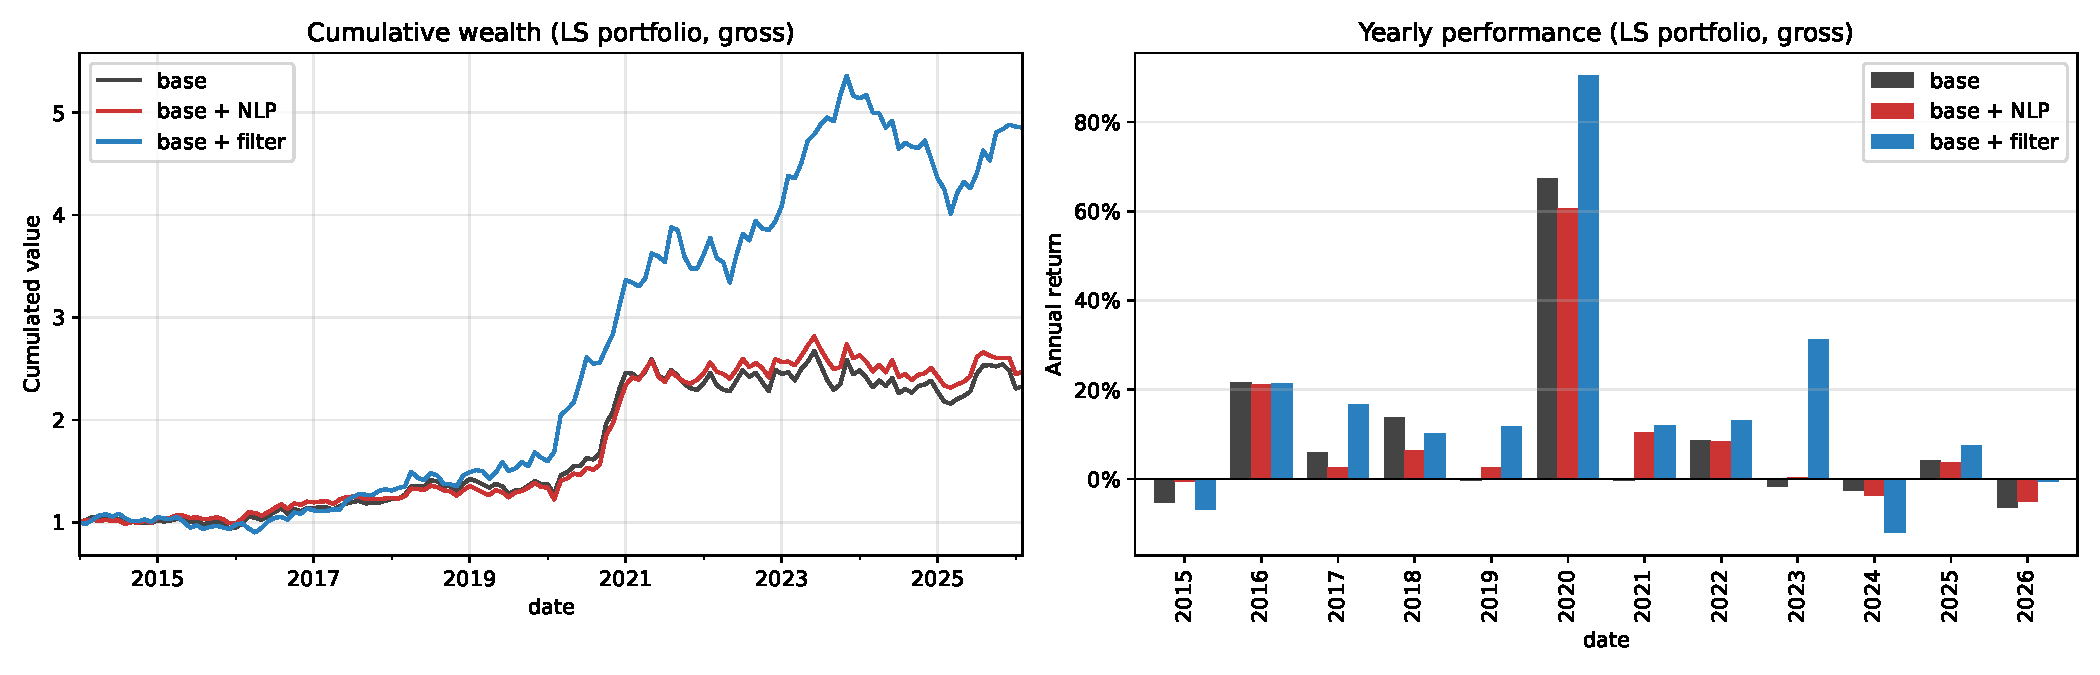
\includegraphics[width=0.7\linewidth]{files/figure_24_1_case_bac-6d7eaa395c4431da788beac29c5d8959.pdf}

The left panel of FIGURE 24.1 plots the cumulative wealth of one dollar invested in each long-short portfolio from January 2014 to the end of the test sample, gross of transaction costs. All three strategies rest on the full 122-characteristic base model; the NLP-feature strategy adds the three real NLP features (LLM 4-dim composite, FinBERT prepared-remarks tone, LM net tone) to the model, while the sentiment-filter strategy overlays the LLM composite on the base book. One dollar grew to 2.33 in the base strategy, 2.47 with the NLP features, and 4.85 with the sentiment filter over the same window, the filter's lead built largely in a handful of strong years (2017, 2019, 2020, and 2023). The right panel decomposes each wealth path into year-on-year performance by reading year-end NAV; the NLP-feature version beats the base in five of the twelve years and the filter in eight of the twelve, and all three fell together in 2024, the concentrated filter book most sharply (-11.7\%), before recovering in 2025.

\subsubsection{Lessons learned}

The first lesson is that NLP features complement, rather than replace, numerical characteristics, and the size of the marginal contribution depends on the baseline. The improvement we observe on the pooled monthly regression from adding three real NLP features to the full 122-characteristic base model is modest because the numerical features already capture a broad set of firm characteristics that are correlated with many aspects of financial text: firms with high earnings growth, for example, also tend to have positive news sentiment, and so the marginal information in the sentiment column is partly redundant. The same NLP features would deliver a substantially larger lift on top of a sparser baseline (a simple OLS on five style factors, say) than on top of a gradient-boosted tree with a richer characteristic stack. This is not a property of NLP, it is a generic property of any incremental feature: the orthogonal component shrinks as the baseline thickens.

Two practical implications follow. Data quality dominates model complexity, in the sense that the coverage, timeliness, and relevance of the underlying text set the upper bound on what any sentiment model can extract; no encoder can recover signal from text that contains none, and the order of priorities for an empirical pipeline is therefore the corpus first, the model second. And small advantages are eaten by transaction costs. The headline long-short improvement we measure on the LLM-covered subuniverse is modest in absolute terms, and a meaningful share of it can be lost if the implied portfolio turnover from a noisier sentiment signal is left unattended. The signal-smoothing and rebalancing-frequency machinery of Chapter 12 is the natural place to manage this, and it should be brought to bear on any production deployment of the features constructed here.

The marginal value of sentiment is also markedly larger where the existing factor environment is weakest. The improvements reported by \cite{kangrga2020factor} for the Asia-Pacific universe, with the information ratio of a multi-factor portfolio rising from 0.45 to 0.74 once a sentiment factor is added, are substantially larger than what we obtain on the US dataset, consistent with the intuition that information disseminates more slowly in markets with thinner analyst coverage. The same principle applies within the US: \cite{hafez2014web} document that news-based predictability is concentrated in small and mid-cap names rather than in the most heavily followed mega-caps. NLP factors are most valuable precisely where the cross-sectional information environment is sparsest, and the empirical reader should expect the lift to scale accordingly when porting the workflow to other regions or to the lower-coverage end of the US cross-section.

A final caveat tempers the headline number. The long-short Sharpe improvement of the case-study overlay reported in Section 24.11, whose novel component is the LLM 4-dim composite scored with a contemporary off-the-shelf model, was obtained with training corpora that extend well beyond the start of our evaluation window, so look-ahead leakage cannot be ruled out by inspection alone. The protocol described in Section 24.4 prescribes a re-run with a \textit{chronologically consistent} encoder \citep{he2025chronologically}, whose weights were trained only on text available before each evaluation date, together with reporting of the profit-mirage diagnostic (the ratio of out-of-sample Sharpe to in-sample Sharpe) alongside the headline number. We flag this re-run as a recommended robustness step rather than execute it here; on the evidence reviewed in Section 24.4 the expected attenuation is moderate (in the range of 10 to 30 percent of the headline Sharpe), but the case study should be considered preliminary until the chronologically consistent replication has been delivered.

\subsubsection{Coding exercise}

\begin{enumerate}
\item Replicate the case study of this chapter using a different ML model
(e.g., random forest or LightGBM instead of XGBoost) and a different set of
base features (e.g., a smaller hand-picked subset of \texttt{mlfi\_us\_data} columns
instead of the full 122-feature panel used in the worked example). Does the
marginal contribution of the NLP features grow as the base feature set is
thinned, as Section 24.12 predicts, and how do the sentiment-filter
thresholds of Section 24.11 affect the gross long-short Sharpe, and how
sensitive is the result to the transaction-cost assumption? Discuss why or why not, and
compare your portfolio statistics to those reported in Section 24.11 of the
chapter.
\end{enumerate}

\subsubsection{References}